\chapter{Implementation}

This chapter not only discusses the technological details of this project but also introduces concrete implementations of two recommender engines as well as the integration of a domain application.

From the very start of this project, it was planned to use free and open-source technologies -- from database management systems to re-usable software libraries. Beside being a well-established best practice in the software programming, the main motivation for this is to avoid software code which is trivial and not contributing to the objectives of the project. It would have gone beyond the scope of this project to build everything from scratch. In fact, by using open-source technology the resulting software code has become very compact and readable.

As a matter of fact, the implemented source code consists of more than 4 thousand lines.

\section{Integration Framework}

The framework has been written in \emph{Python} and is entirely object-oriented. The source code is grouped into modules. The code structure is as follows:

\begin{description}
    \item[api] implements the \emph{application programming interface (API)}.
    \item[config] holds the configuration file as well as the \emph{XML schema definition (XSD)}.
    \item[core] provides classes processing the configuration file as well as taxonomies. Furthermore, the engine submodule implements abstract base classes for engine adapters.
    \item[engines] contain engine adapter classes. In this case, it has adapters for the engines \emph{in-common}, \emph{item-similarity} and the hybrid engine \emph{weighted}.
    \item[log] has log files which are useful to troubleshoot problems.
    \item[tests] define a unit test suite.
    \item[worker] implements the workers for Event and Recommend.
    \item[api.wsgi] is the WSGI server loaded by Apache and runs the API.
    \item[config.py] loads the configuration and makes it available for other classes in the source code.
    \item[monitor.py] reloads the WSGI server when local changes to Python files were detected. The author of this particular file has been acknowledged in the source code.
    \item[requirements.txt] holds the name and versions of Python libraries the framework is depending on. It is used by the Python dependency manager \emph{pip}.
\end{description}

The framework has no persistence at all and thus does not utilise a database management system. As mentioned in the section \ref{architecture-integration-framework}, it operates as middleware between domain and recommender engines, therefore relying on those to handle their persistence requirements. As far as the framework is concerned, there is no need or purpose to persist data.

\subsection{API}

The \emph{application programming interface (API)} of the framework is based on the popular, so-called micro web application framework \emph{Flask}. The notation of micro refers to the fact, that Flask is very minimal and has almost no constraints on other technologies such as database management systems.

\begin{figure}[ht]
    \inputminted{py}{./includes/source/framework/api/event.py}
    \caption{Event API (Code Listing)}
    \label{fig:implementation-framework-api-event}
\end{figure}

The API uses the \emph{JavaScript Object Notation (JSON)} format data and is served by the open-source web server \emph{Apache} as a virtual host through the \emph{web server gateway interface (WSGI)} and listens to requests at \url{http://api.msc.koklu.me}.

It was originally proposed to use \emph{NodeJS} and \emph{express} for the API. However it was later chosen to be Python for the following reasons: First, the rest of the framework was going to be in Python and the task queue management software \emph{Celery}, which is going to be introduced in the next section, is working most elegantly with Python. Second, there was no exclusive benefit by implementing the API in NodeJS instead of Flask. Third, Flask provides the same minimalistic approach to defining routes as express.

\subsection{Worker \& Task Queue}

The project relies on the task queue system \emph{Celery} to establish an asynchronous and selectively synchronous communication between API and workers. Celery is written in Python and supports multiple brokers such as \emph{RabbitMQ} and \emph{Beanstalk}. The former is used as broker in this project.



\begin{figure}[ht]
    \inputminted{py}{./includes/source/framework/worker/event.py}
    \caption{Event Worker (Code Listing)}
    \label{fig:implementation-framework-worker}
\end{figure}

The Event API is calling its worker asynchronously -- thus not waiting for a response (\emph{queue \& forget}) -- whereas the Recommend API is doing that synchronously. Figure \ref{fig:implementation-framework-worker} lists the source code of the event worker which is upon request going through all recommenders subscribed to the given event and calls the configured event method on the engine adapter.

It was initially intended to use RabbitMQ natively as a message queue implementing the \emph{advanced message queuing protocol (AMQP)}. However, while looking for RabbitMQ client libraries and elegant ways to manage the overhead of using message queues for distributing tasks, Celery was discovered which abstracts that complexity completely. Tasks can be run as if they are regular methods in the source code (see line 3 of Figure \ref{fig:implementation-framework-api-event}).

Flower is an administrative interface for Celery providing a real-time monitor and can be accessed at \url{http://flower.msc.koklu.me} (Figure \ref{fig:implementation-framework-flower}).

\begin{figure}[ht]
    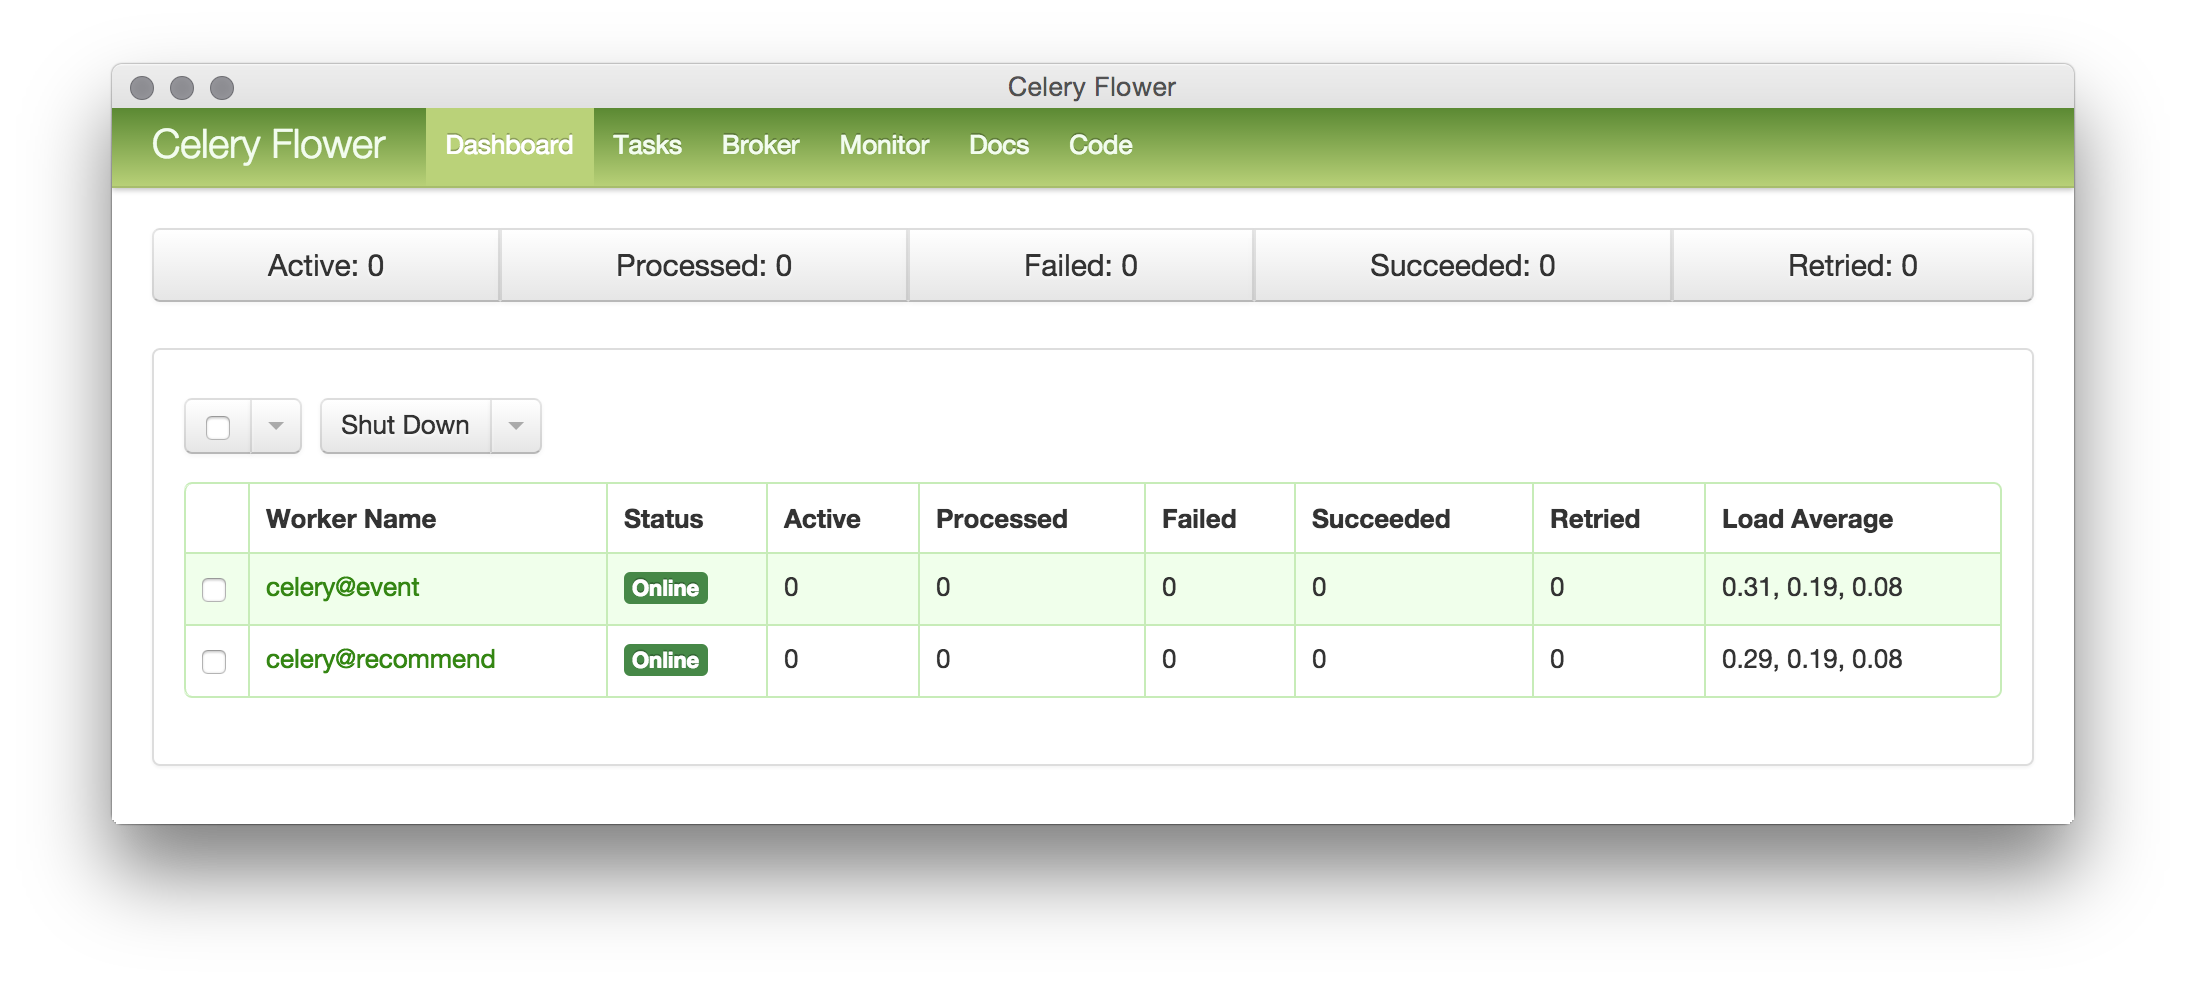
\includegraphics[width=\textwidth,center]{screens/flower.png}
    \caption{Flower for Celery (Screenshot)}
    \label{fig:implementation-framework-flower}
\end{figure}

\subsection{Configuration}

\begin{figure}[ht!]
    \begin{minted}{xml}
<?xml version="1.0" encoding="UTF-8"?>
<config xmlns:xsi="http://www.w3.org/2001/XMLSchema-instance" xsi:noNamespaceSchemaLocation="./config.xsd">
    <recommenders>
        <!-- [...] -->
        <recommender name="similar_products_in_basket" engine="item_similarity">
            <on event="saved_product" do="post" />
            <on event="deleted_product" do="delete" />
            <taxonomy inherit="base">
                <taxon name="item_id">sku</taxon>
                <taxon name="itemIds">sku</taxon>
                <taxon name="attributes">data</taxon>
            </taxonomy>
        </recommender>
        <hybrid_recommender name="interesting_products" engine="weighted">
            <components>
                <component name="views" recommender="common_products_viewed" />
                <component name="wishlists" recommender="common_products_wishlisted" />
            </components>
            <settings>
                <weight>
                    <views>0.25</views>
                    <wishlists>0.75</wishlists>
                </weight>
            </settings>
        </hybrid_recommender>
    </recommenders>
    <taxonomies>
        <taxonomy name="base">
            <taxon name="limit">limit</taxon>
        </taxonomy>
        <!-- [...] -->
    </taxonomies>
    <engines>
        <engine name="in_common">
            <settings>
                <base_url>http://localhost:8080/</base_url>
            </settings>
        </engine>
        <!-- [...] -->
    </engines>
    <!-- [...] -->
</config>
    \end{minted}
    \caption{Shortened XML Configuration (Code Listing)}
    \label{fig:implementation-framework-configuration}
\end{figure}

Figure \ref{fig:implementation-framework-configuration} shows a shortened configuration file of the framework and is explained as follows:

\begin{description}
    \item[recommenders/recommender] defines a recommender by name and the engine to be used. Furthermore it has a list of events it subscribes to (\texttt{on}) where the \texttt{do} attribute refers to the method of the engine adapter to be called when the event occurs. A recommender also defines a taxonomy which usually inherits from a global taxonomy.
    \item[recommenders/hybrid_recommender] defines a hybrid recommender which consists of two or more components. It may also have some settings which can be accessed by the engine adapter.
    \item[taxonomies/taxonomy] defines a global taxonomy which is a data contract and terminology mapper between domain and recommender engines. It may inherit from another taxonomy. A taxonomy consists of \texttt{taxon} elements which describe a single mapping.
    \item[engines/engine] holds settings for engines.
    \item[settings] hold global settings of the framework such as connection details for Celery.
\end{description}

The project also provides an \emph{XML schema definition (XSD)} which can be used to validate a framework configuration.

\subsection{Engine Adapters}
\label{implementation-framework-engine-adapter}

\begin{figure}[!ht]
    \inputminted{py}{./includes/source/framework/engines/item\string_similarity.py}
    \caption{Item-Similarity Engine Adapter (Code Listing)}
    \label{fig:implementation-framework-engine-adapter}
\end{figure}

\emph{Engine adapters} are thin clients to recommender engines. The formal requirement is that they implement a \texttt{recommend} method as well as methods used in event subscriptions. Other than that, it is completely flexible in how the interaction with the engine happens. For convenience, the abstract base class provides a RESTful skeleton which is used by the engine adapters implemented in this project such as the \emph{item-similarity} adapter (see Figure \ref{fig:implementation-framework-engine-adapter}). Engine adapters have access to engine settings defined in the configuration file such as a \emph{uniform resource locator (URL)} for the engine.

Engine adapters for hybrid engines are more than just thin clients. Their formal requirement is to implement a \texttt{recommend} method but has no event methods. In this method they have full flexibility on how to make use of the components. Figure \ref{fig:implementation-framework-hybrid-engine-adapter} shows the implementation of the \emph{weighted} hybrid engine adapter.

\begin{figure}[!ht]
    \begin{minted}{py}
from collections import OrderedDict
from core.engine.hybrid import HybridEngine as ParentHybridEngine

class HybridEngine(ParentHybridEngine):
    def recommend(self, body):
        return self.merge(self.apply_weight(self.get_results(body)))

    def get_results(self, body):
        results = {}
        for name, component in self.components.iteritems():
            result = component.recommend(body, True)
            if result:
                results[name] = result

        return results

    # [...] implementations of merge and apply_weight
    \end{minted}
    \caption{Weighted Hybrid Engine Adapter (Code Listing)}
    \label{fig:implementation-framework-hybrid-engine-adapter}
\end{figure}



\section{Engines}

\subsection{Collaborative Recommender Engine: In-Common}

This recommender engine has a collaborative filtering approach and basically performs recommendations as shown in Figure \ref{fig:intro-techniques-collaborative}: \texttt{recommend items which other users, who have experienced the same items as the given user, have experienced but the given user has not yet}. The fundamental idea behind this engine is to parametise the aforementioned query. There are four parameters in this query: \emph{subject} such as a user or customer, \emph{object} such as a product, \emph{relationship} such as viewed or favourited and \emph{subject ID} such as the current user.

The engine is processing events and recommendation requests in real-time. Although it persists data, it is data-agnostic -- in other words, it knows how the data is structured but does not require knowledge about the data itself.

This engine has been written in \emph{Go} -- a statically typed language developed at \emph{Google} in 2007. \citet{pike12} explains the motivation behind building Go:

\begin{adjustwidth}{1cm}{}
\emph{``The goals of the Go project were to eliminate the slowness and clumsiness of software development at Google, and thereby to make the process more productive and scalable. The language was designed by and for people who write -- and read and debug and maintain -- large software systems.''}
\end{adjustwidth}

As far as this project is concerned, there was much interest in using a statically typed, compiled language in one of its subprojects to accommodate the \emph{technological unbiasedness} property of the framework. The code is organised in packages as follows:

\begin{description}
    \item[api] implements the \emph{application programming interface (API)}.
    \item[engine] provides capabilities of the engine, yet at the present time acts merely as an interface to the graph functions.
    \item[graph] performs operations and queries on the database.
    \item[log] holds log files for troubleshooting.
    \item[model] defines data models such as a recommendation request or relationship.
    \item[util] offers a few utility functions.
\end{description}

Go has out-of-the-box support for building a API documentation for Go source code. The documentation for the In-Common recommender engine can be found here: \url{http://godoc.org/github.com/halk/in-common}.

\subsubsection{API}

The API of this engine is built based on the \texttt{http} package of Go. The following services are available:

\begin{description}
    \item[POST /event] processes a new event and expects a JSON-encoded payload consisting of \texttt{subject}, \texttt{subject_id}, \texttt{object}, \texttt{object_id} and \texttt{relationship}.
    \item[DELETE /event] deletes an event and expects the same JSON-encoded model as above.
    \item[GET /recommend] receives a recommendation request with \texttt{subject}, \texttt{subject_id}, \texttt{object}, \texttt{relationship} and \texttt{limit} \emph{GET} parameters but returns a JSON-encoded list of recommended \texttt{object IDs}. The parameter \texttt{limit} specifies how many recommendations should be queried and returned.
\end{description}

\subsubsection{Data Representation}

\begin{figure}[ht]
    \includegraphics[width=250pt,center]{implementation/incommon\string_nodes.pdf}
    \caption{In-Common Data Representation (Diagram)}
    \label{fig:implementation-incommon-nodes}
\end{figure}

The data representation is the heart of this engine. As proposed in the project proposal, the graphical database management system \emph{Neo4j} has been used for persistence. The graphical representation is ideal for events since they can be perceived as a relationship between two nodes -- subject and object (Figure \ref{fig:implementation-incommon-nodes}). Hence, the recommendation request is just a query against this graph (Figure \ref{fig:implementation-incommon-recommendation-query}).

All nodes and relationships are stored in the same database, even if the recommenders and their data defined in the framework are different. This is in that sense not an issue, since as long as the recommenders are not using the same subject and object labels, there is no collaboration happening between those.

\begin{figure}[!ht]
    \begin{minted}{go}
cq := neoism.CypherQuery{
    Statement: fmt.Sprintf(
        `
            MATCH (subject:%[1]s)-[:%[2]s]->(%[3]s)<-[:%[2]s]-(%[1]s)-[r:%[2]s]->(object:%[3]s)
            WHERE subject.id = {subjectId} AND NOT((subject)-[:%[2]s]->(object))
            RETURN object.id, COUNT(r) AS weight
            ORDER BY weight DESC
            LIMIT %[4]d
      `,
        util.UpperCaseFirst(rq.Subject), strings.ToUpper(rq.Relationship),
        util.UpperCaseFirst(rq.Object), rq.Limit,
    ),
    Parameters: neoism.Props{"subjectId": rq.SubjectID},
    Result:     &res,
}
    \end{minted}
    \caption{In-Common Recommendation Query (Code Listing)}
    \label{fig:implementation-incommon-recommendation-query}
\end{figure}

\subsection{Content-Based Recommender Engine: Item-Similarity}

The \emph{Item-Similarity} recommender engine adopts the content-based filtering approach which computes the similarity of items by comparing their features.

This engine has been written in \emph{PHP: Hypertext Preprocessor (PHP)} following the \emph{object-oriented programming (OOP)} paradigm and is based on the micro web framework \emph{Silex} -- similar to \emph{Flask} used by the framework. The source code structure is as follows:

\begin{description}
    \item[config] contains very minimal configuration such as the \emph{data source name (DSN)} -- the connection details -- to the database.
    \item[log] has some log files for troubleshooting.
    \item[src/Koklu/Entity] defines entity model classes such as an \texttt{Item}.
    \item[src/Koklu/Model] holds classes to manage and recommend items as well as the similarity algorithm \texttt{TanimotoCoefficient} which was discussed in the project proposal.
    \item[src/Koklu/Repository] interacts with the database.
    \item[src/Koklu/Service] implements a service which is a proxy for the classes above and is made available to the API.
    \item[src/app.php] defines the application and API services.
    \item[src/bootstrap.php] initialises essential resources and is also used to initialise the unit tests.
    \item[tests] contain the unit tests.
    \item[web] provides a front controller which loads the application and makes it publicly accessible.
\end{description}

\subsubsection{API}

In contrast to the API of the \emph{In-Common} recommender engine, this engine introduces the concept of collections to separate data of different recommenders using this engine. This is due to the fact that this engine computes recommendations relying on all available data. Collections limit that spectrum to the data of one recommender e.g. \texttt{similar_products_in_basket}.

\begin{description}
    \item[POST /\{collection\}] creates or updates an item and expects a JSON-encoded payload consisting of \texttt{item_id} and \texttt{attributes}. The latter is an arbitrary JSON object containing any data to be considered while calculating the similarity.
    \item[DELETE /\{collection\}/\{itemId\}] deletes an item.
    \item[GET /\{collection\}] receives a recommendation request with \texttt{itemIds} and \texttt{limit} \emph{GET} parameters but returns a JSON-encoded list of identifiers of recommended items. The GET parameter \texttt{itemIds} can contain more than one item ID. The parameter \texttt{limit} specifies how many recommendations should be queried and returned.
\end{description}

\subsubsection{Data Representation}

The \emph{Item-Similarity} engine uses the document-oriented, \emph{NoSQL} database management system \emph{MongoDB}. NoSQL refers to a variety of data modelling and retrieval methods which differ from traditional, relational database management systems such as \emph{MySQL}. MongoDB stores data as schemaless, JSON documents in collections which is ideal for this use-case as the engine has no knowledge about the schema of the item features -- henceforth referred to as \emph{attributes}. The engine makes use of \emph{Doctrine MongoDB Object Document Mapper (ODM)} to interact with the MongoDB database in an object-oriented way.

Another benefit is the support for subdocuments which allows nested data. Figure \ref{fig:implementation-itemsimilarity-entity} shows the following document structure for the \emph{Item} entity: \texttt{id} is a unique identifier of the item, usually the identifier passed through from the domain application, \texttt{attributes} holds a \emph{key-value} representation of the item features whereas \texttt{similar} contains \emph{Similar} entities which consists of a reference to another item and a similarity score.

\begin{figure}[!ht]
    \def\arraystretch{1.5}
    \centering
    \begin{tabular}{|
    >{\columncolor[HTML]{CBCEFB}}l |l|l|l|}
    \hline
    {\textbf{id}}                                                   & \multicolumn{3}{l|}{3}                                                                               \\ \hline
    \cellcolor[HTML]{CBCEFB}                                   & \cellcolor[HTML]{ECF4FF}{\emph{weight}}                  & \multicolumn{2}{l|}{3}                       \\ \cline{2-4} 
    \cellcolor[HTML]{CBCEFB}                                   & \cellcolor[HTML]{ECF4FF}{\emph{height}}                  & \multicolumn{2}{l|}{2}                       \\ \cline{2-4} 
    \multirow{-3}{*}{\cellcolor[HTML]{CBCEFB}{\textbf{attributes}}} & \cellcolor[HTML]{ECF4FF}{\emph{color}}                   & \multicolumn{2}{l|}{red}                     \\ \hline
    \cellcolor[HTML]{CBCEFB}                                   & \cellcolor[HTML]{BBDAFF}                              & \cellcolor[HTML]{ECF4FF}{\emph{item}}  & Ref(1) \\ \cline{3-4} 
    \cellcolor[HTML]{CBCEFB}                                   & \multirow{-2}{*}{\cellcolor[HTML]{BBDAFF}{\textbf{\emph{0}}}} & \cellcolor[HTML]{ECF4FF}{\emph{score}} & 2.5    \\ \cline{2-4} 
    \cellcolor[HTML]{CBCEFB}                                   & \cellcolor[HTML]{BBDAFF}                              & \cellcolor[HTML]{ECF4FF}{\emph{item}}  & Ref(2) \\ \cline{3-4} 
    \multirow{-4}{*}{\cellcolor[HTML]{CBCEFB}{\textbf{similar}}}    & \multirow{-2}{*}{\cellcolor[HTML]{BBDAFF}{\textbf{\emph{1}}}} & \cellcolor[HTML]{ECF4FF}{\emph{score}} & 0.4    \\ \hline
    \end{tabular}
    \caption{Item Entity Model (Table)}
    \label{fig:implementation-itemsimilarity-entity}
\end{figure}

An item is created by instantiating an \emph{Item} entity and iterating through all other items in the collection; for each item the similarity is calculated and a \emph{Similar} entity referencing this item added to the created item as well as a \emph{Similar} entity referencing the created item to the compared item. An item is updated by removing and recreating. An item is removed by deleting the \emph{Item} entity and all \emph{Similar} entities referencing to it, which are subdocuments of other items. Figure \ref{fig:implementation-itemsimilarity-similarity} illustrates this as a matrix with the red column and row relating to data added or removed.

\begin{figure}[!ht]
    \def\arraystretch{1.5}
    \centering
    \begin{tabular}{|
    >{\columncolor[HTML]{BBDAFF}}c |c|c|c|
    >{\columncolor[HTML]{FD6864}}c |}
    \hline
    {\textbf{\emph{items}}} & \cellcolor[HTML]{BBDAFF}{\textbf{1}} & \cellcolor[HTML]{BBDAFF}{\textbf{2}} & \cellcolor[HTML]{BBDAFF}{\textbf{3}} & \cellcolor[HTML]{BBDAFF}{\textbf{4}} \\ \hline
    {\textbf{1}} & \diagbox[width=0.8cm, height=0.8cm]{}{} & 0.3 & 1.2 & 0.7\\ \hline
    {\textbf{2}} & 0.3 & \diagbox[width=0.8cm, height=0.8cm]{}{} & 0.8 & 0.2\\ \hline
    {\textbf{3}} & 1.2 & 0.8 & \diagbox[width=0.8cm, height=0.8cm]{}{} & 0.5\\ \hline
    {\textbf{4}} & \cellcolor[HTML]{FD6864}0.7 & \cellcolor[HTML]{FD6864}0.2 & \cellcolor[HTML]{FD6864}0.5 & \diagbox[width=0.8cm, height=0.8cm]{}{}\\ \hline
    \end{tabular}
    \caption{Similarity Matrix (Table)}
    \label{fig:implementation-itemsimilarity-similarity}
\end{figure}

As the similarity of items is computed at the time of change rather than request, the recommendation query is very straightforward and fetches items referenced by the \emph{Similar} entities sorted by score in a descending order. As the recommendation request can be based on more than one item, a simple \texttt{find} query is not sufficient and an \texttt{aggregate} query was required. Doctrine ODM does not provide an interface for that yet, thus the engine queries MongoDB directly (Figure \ref{fig:implementation-itemsimilarity-recommendation-query}).

\begin{figure}[!ht]
    \begin{minted}{php}
/**
 * @param string   $collection
 * @param array    $forItems
 * @param int|bool $limit
 * @return array
 */
public function findSimilarItems($collection, array $forItems, $limit)
{
    $pipeline = [
        ['$match' => ['_id' => ['$in' => $forItems]]],
        ['$unwind' => '$similar'],
        ['$group' => ['_id' => '$similar.item', 'score' => ['$max' => '$similar.score']]],
        ['$sort' => ['score' => -1]]
    ];

    if ($limit !== false) {
        $pipeline[] = ['$limit' => (int) $limit];
    }

    return $this->getDocumentManager()->getDocumentDatabase($this->getClassName())->getMongoDB()
        ->selectCollection($collection)
        ->aggregate($pipeline);
}
    \end{minted}
    \caption{Item-Similarity Recommendation Query (Code Listing)}
    \label{fig:implementation-itemsimilarity-recommendation-query}
\end{figure}

\subsubsection{Tanimoto Coefficient}

\begin{figure}[ht]
    \[T = \frac{N_{ab}}{(N_a + N_b - N_{ab})}\]
    \caption[Tanimoto Coefficient]{Tanimoto Coefficient where \(N_a\) respectively \(N_b\) is the count of properties of \(a\) respectively \(b\) and \(N_{ab}\) is the count of intersecting properties.}
    \label{fig:implementation-itemsimilarity-tanimoto}
\end{figure}

The \emph{Tanimoto coeffcient} describes the similarity of two \emph{sets} as shown in Figure \ref{fig:implementation-itemsimilarity-tanimoto} \cite{segaran07}. An intersection of properties refer to all properties which exist in both sets.

Since the attribute data of items is a \emph{hash map}, it needs to be converted into a set. A hash map can be seen as a key-value table whereas a set is just a list of properties. A typical way to convert a hash map into a set is by discarding its keys. However, this is not a solution in this case. Given the following two hash maps: \texttt{A = \{width: 3, height: 2\}} and \texttt{A = \{width: 4, height: 3\}}, discarding would produce as follows: \texttt{A = [3, 2]} and \texttt{B = [4, 3]}. The Tanimoto coefficient would assume that they have at least one similar property, although the \texttt{3} is actually from different properties. This engine solves this by concatenating the key and a string representation of the value. The converted sets now look like this: \texttt{A = [width3, height2]} and \texttt{B = [width4, height3]}, thus have no similarity. Another problem is that attributes do not only contain alphanumeric values but also lists, e.g.: \texttt{A = \{tags: red,circular\}} and \texttt{B = \{tags: green,circular\}}. Although the properties do not match exactly, both items are \texttt{circular}. A solution is to repeat the key and value concatenation for each list item: \texttt{A = [tagsred, tagscircular]} and \texttt{B = [tagsgreen, tagscircular]}.

Figure \ref{fig:implementation-itemsimilarity-tanimotocode} lists the implementation of the Tanimoto coefficient in this engine.

\begin{figure}[!ht]
    \inputminted{php}{./includes/source/engines/itemSimilarity/src/Koklu/Model/Similarity/TanimotoCoefficient.php}
    \caption{Tanimoto Coefficient Implementation (Code Listing)}
    \label{fig:implementation-itemsimilarity-tanimotocode}
\end{figure}

\subsection{Hybrid Recommender: Weighted}

Returning to the hybrid recommender engine \emph{weighted} which has already been touched on in section \ref{implementation-framework-engine-adapter} and illustrated in Figure \ref{fig:implementation-framework-hybrid-engine-adapter}, this section provides a brief explanation on how the scores are combined by weighting. Weighting in this scenario relates to preferring the results of a  component over the others.

This particular weighted implementation first fetches recommendations from each component recommender engine. The recommendations come with a score attached to it -- a numeric value indicating a level of preference over the other recommendations. The engine has a weight configured as a setting which is preferably a value between 0 and 1 so that the sum of all weights is 1. While looping through each component's recommendations, the score of the recommendation is multiplied with the respective weight for the component (see Figure \ref{fig:implementation-weighted}). This has a dampening effect on the scores. Then, the sets of recommendations are merged into one set. If a recommendation exists in more than one set, then the scores added together. Finally, this merged set is sorted by score in descending order.

\begin{figure}[!ht]
    \def\arraystretch{1.5}
    \begin{tabular}{|
    >{\columncolor[HTML]{ECF4FF}}l |
    >{\columncolor[HTML]{ECF4FF}}r |r|r|r|r|}
    \hline
    \cellcolor[HTML]{BBDAFF}{\color[HTML]{000000} {\textbf{recommender}}} & \multicolumn{1}{c|}{\cellcolor[HTML]{BBDAFF}{\color[HTML]{000000} {\textbf{weight}}}} & \multicolumn{1}{c|}{\cellcolor[HTML]{BBDAFF}{\color[HTML]{000000} {\textbf{Item \#1}}}} & \multicolumn{1}{c|}{\cellcolor[HTML]{BBDAFF}{\color[HTML]{000000} {\textbf{Item \#2}}}} & \multicolumn{1}{c|}{\cellcolor[HTML]{BBDAFF}{\color[HTML]{000000} {\textbf{Item \#3}}}} & \multicolumn{1}{c|}{\cellcolor[HTML]{BBDAFF}{\color[HTML]{000000} {\textbf{Item \#4}}}} \\ \hline
    viewed\_products & 0.25 & 1 & 0.75 & 0.5 & 1 \\ \hline
    wishlisted\_products & 0.75 & 0.5 & 0.95 & 0.3 & 1 \\ \hline
    {\textbf{\emph{weighted recommender}}} & {\textbf{\emph{1}}} & {\textbf{\emph{0.625}}} & {\textbf{\emph{0.9}}} & {\textbf{\emph{0.35}}} & {\textbf{\emph{1}}} \\ \hline
    \end{tabular}
    \caption{Sample Calculation of Weighted Hybrid Recommender Engine (Table)}
    \label{fig:implementation-weighted}
\end{figure}

\section{Demo Domain System: Magento}

Section \ref{architecture-domain-applications} discussed the definition and characteristics of domain applications which are founded on extensive domain knowledge. Although the focus of the project is on the framework and recommender engines, it was clear from the beginning that they needed to be trialled and demonstrated on a complex domain application. Since e-commerce websites are amongst the major users of recommender engines, demonstrating the work on an e-commerce system was of symbolic importance. As proposed, the e-commerce software \emph{Magento} has been used for this. \citet{aheadworks14} analysed \emph{Alexa}'s 1 million top sites index and found that Magento was the leading open-source e-commerce software with a market share of 30 per cent in 2014. Magento is written in \emph{PHP: Hypertext Preprocessor (PHP)} and relies on the relational database management system \emph{MySQL}. In fact, this project uses \emph{Percona Server} as an enhanced, drop-in replacement for MySQL to have better performance.

\begin{figure}[!ht]
    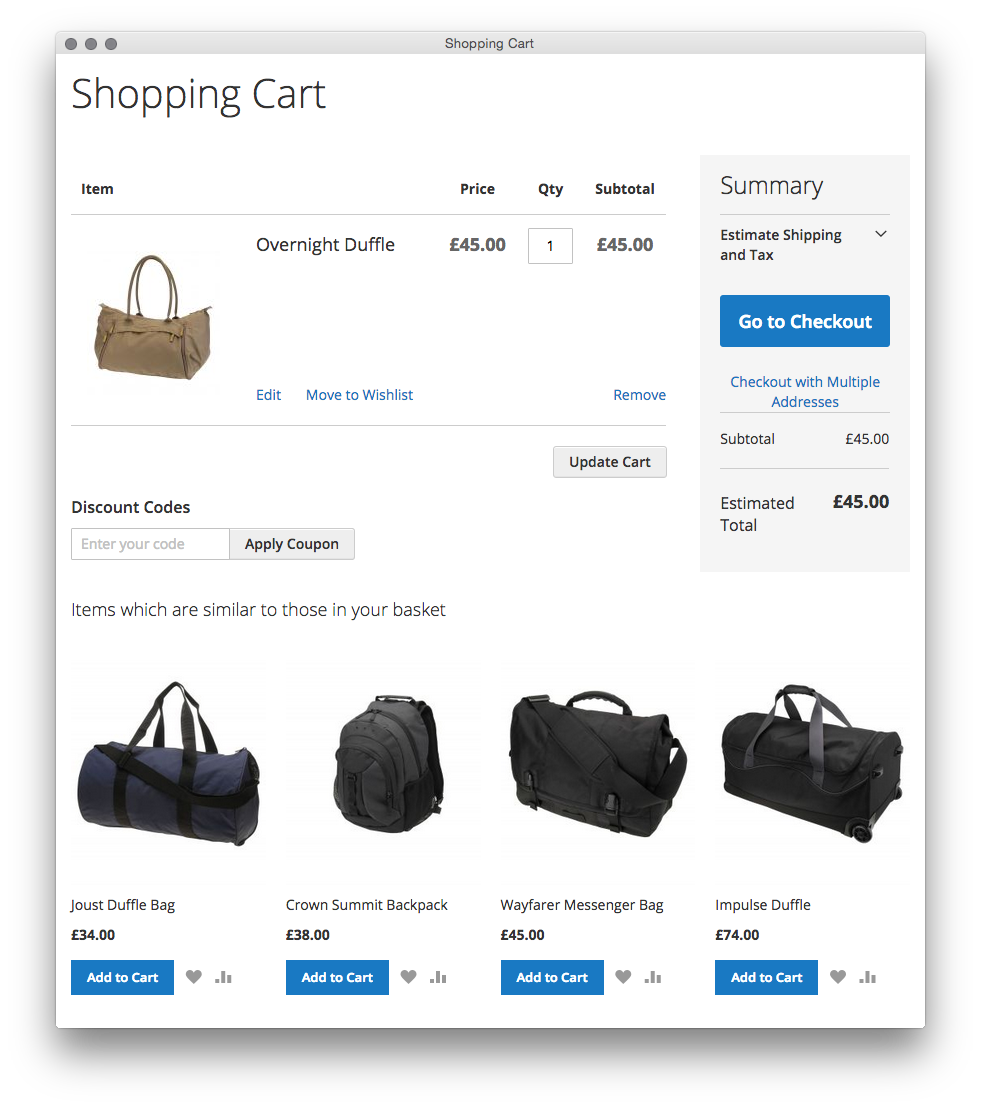
\includegraphics[width=\textwidth,center]{screens/basket.png}
    \caption{Content-Based Recommendation (Screenshot)}
    \label{fig:implementation-magento-basket}
\end{figure}

The authors of Magento are working on a full rewrite of their platform called Magento2 to be released late 2015. This project uses the first release candidate published in March 2015. Albeit Magento2 comes with fundamental technical changes, they do not necessarily make a difference to the purposes of demonstration. Nonetheless the support of the dependency manager \emph{Composer} was principally important to distinct between custom code from that supplied by the application. Secondly, the sample data generator was useful to demo with realistic data.

The source code written for this project is structured as follows:

\begin{description}
    \item[app/code/Koklu/Event] module handles observing and processing of events.
    \item[app/code/Koklu/MasterData] module complements the Event module by handling master data related events and full exports.
    \item[app/code/Koklu/Recommender] modules queries and display recommendations as well as providing a client for the recommendation framework.
    \item[dev/shell/masterdata.php] script runs a full export of master data to the framework.
    \item[lib/internal/Koklu/Rest/Json] fixes a bug in the Zend library which sometimes omits setting the HTTP header \emph{Accept-Encoding} to \emph{JSON}.
\end{description}

\subsection{Events}
\label{implementation-magento-events}

Magento comes with an event subsystem in which observers can subscribe to various events -- from very low-level to very specific functions. This helped to keep the required code clean and short.

The following cases are recorded and posted to the framework as events:

\begin{itemize}
\item \emph{Customer views a product}
\item \emph{Customer adds or removes a product to their wish list}
\item \emph{Customer adds a product to their basket}
\end{itemize}

There are more cases which are interesting in an e-commerce context such as the actual purchase of items. The aforementioned cases have been symbolically chosen as they do not require too many steps to reproduce. By contrast, a checkout on Magento is a longer process which requires documentation and can be time-consuming on slow development environments.

Finally, the customer identification is part of the data for almost all events. A customer who has not logged in yet gets a \emph{visitor ID} assigned to by Magento. This allows behavioural analysis and production of recommendations even for logged out users. Once they log in, the \emph{customer ID} can be used so that the recommendations can source from historic sessions. In order to troubleshoot any issues, all requests and responses to the event API of the framework are logged in a file.

\subsection{Master Data}
\label{implementation-magento-masterdata}

The master data is exceptionally important for content-based recommenders as they source their recommendations from similarities between item features. In the Magento context, master data refers to the product catalogue and is sent to the framework as regular events. Again, the event subsystem allows to observer product catalogue changes and notify the framework in real-time. On first run or if explicitly wished, the catalogue data can be exported as a whole with a command-line script. This is known as full export and the data is transmitted in batches.

Magento implements an \emph{entity-attribute-value (EAV)} model. \emph{Entities} are a type of product such as books and are called \emph{attribute sets} in Magento. \emph{Attributes} are fields within a product catalogue and have a value type such as text or numeric amounts. Values can be entered freely or chosen from an editable list. The EAV model basically describes that although the number of attributes in a catalogue is vast, only a subset of those are relevant and applicable to an entity -- in practice it means that an attribute \emph{``number of pages''} is relevant for a book but not necessarily for a phone.

\begin{figure}[!ht]
    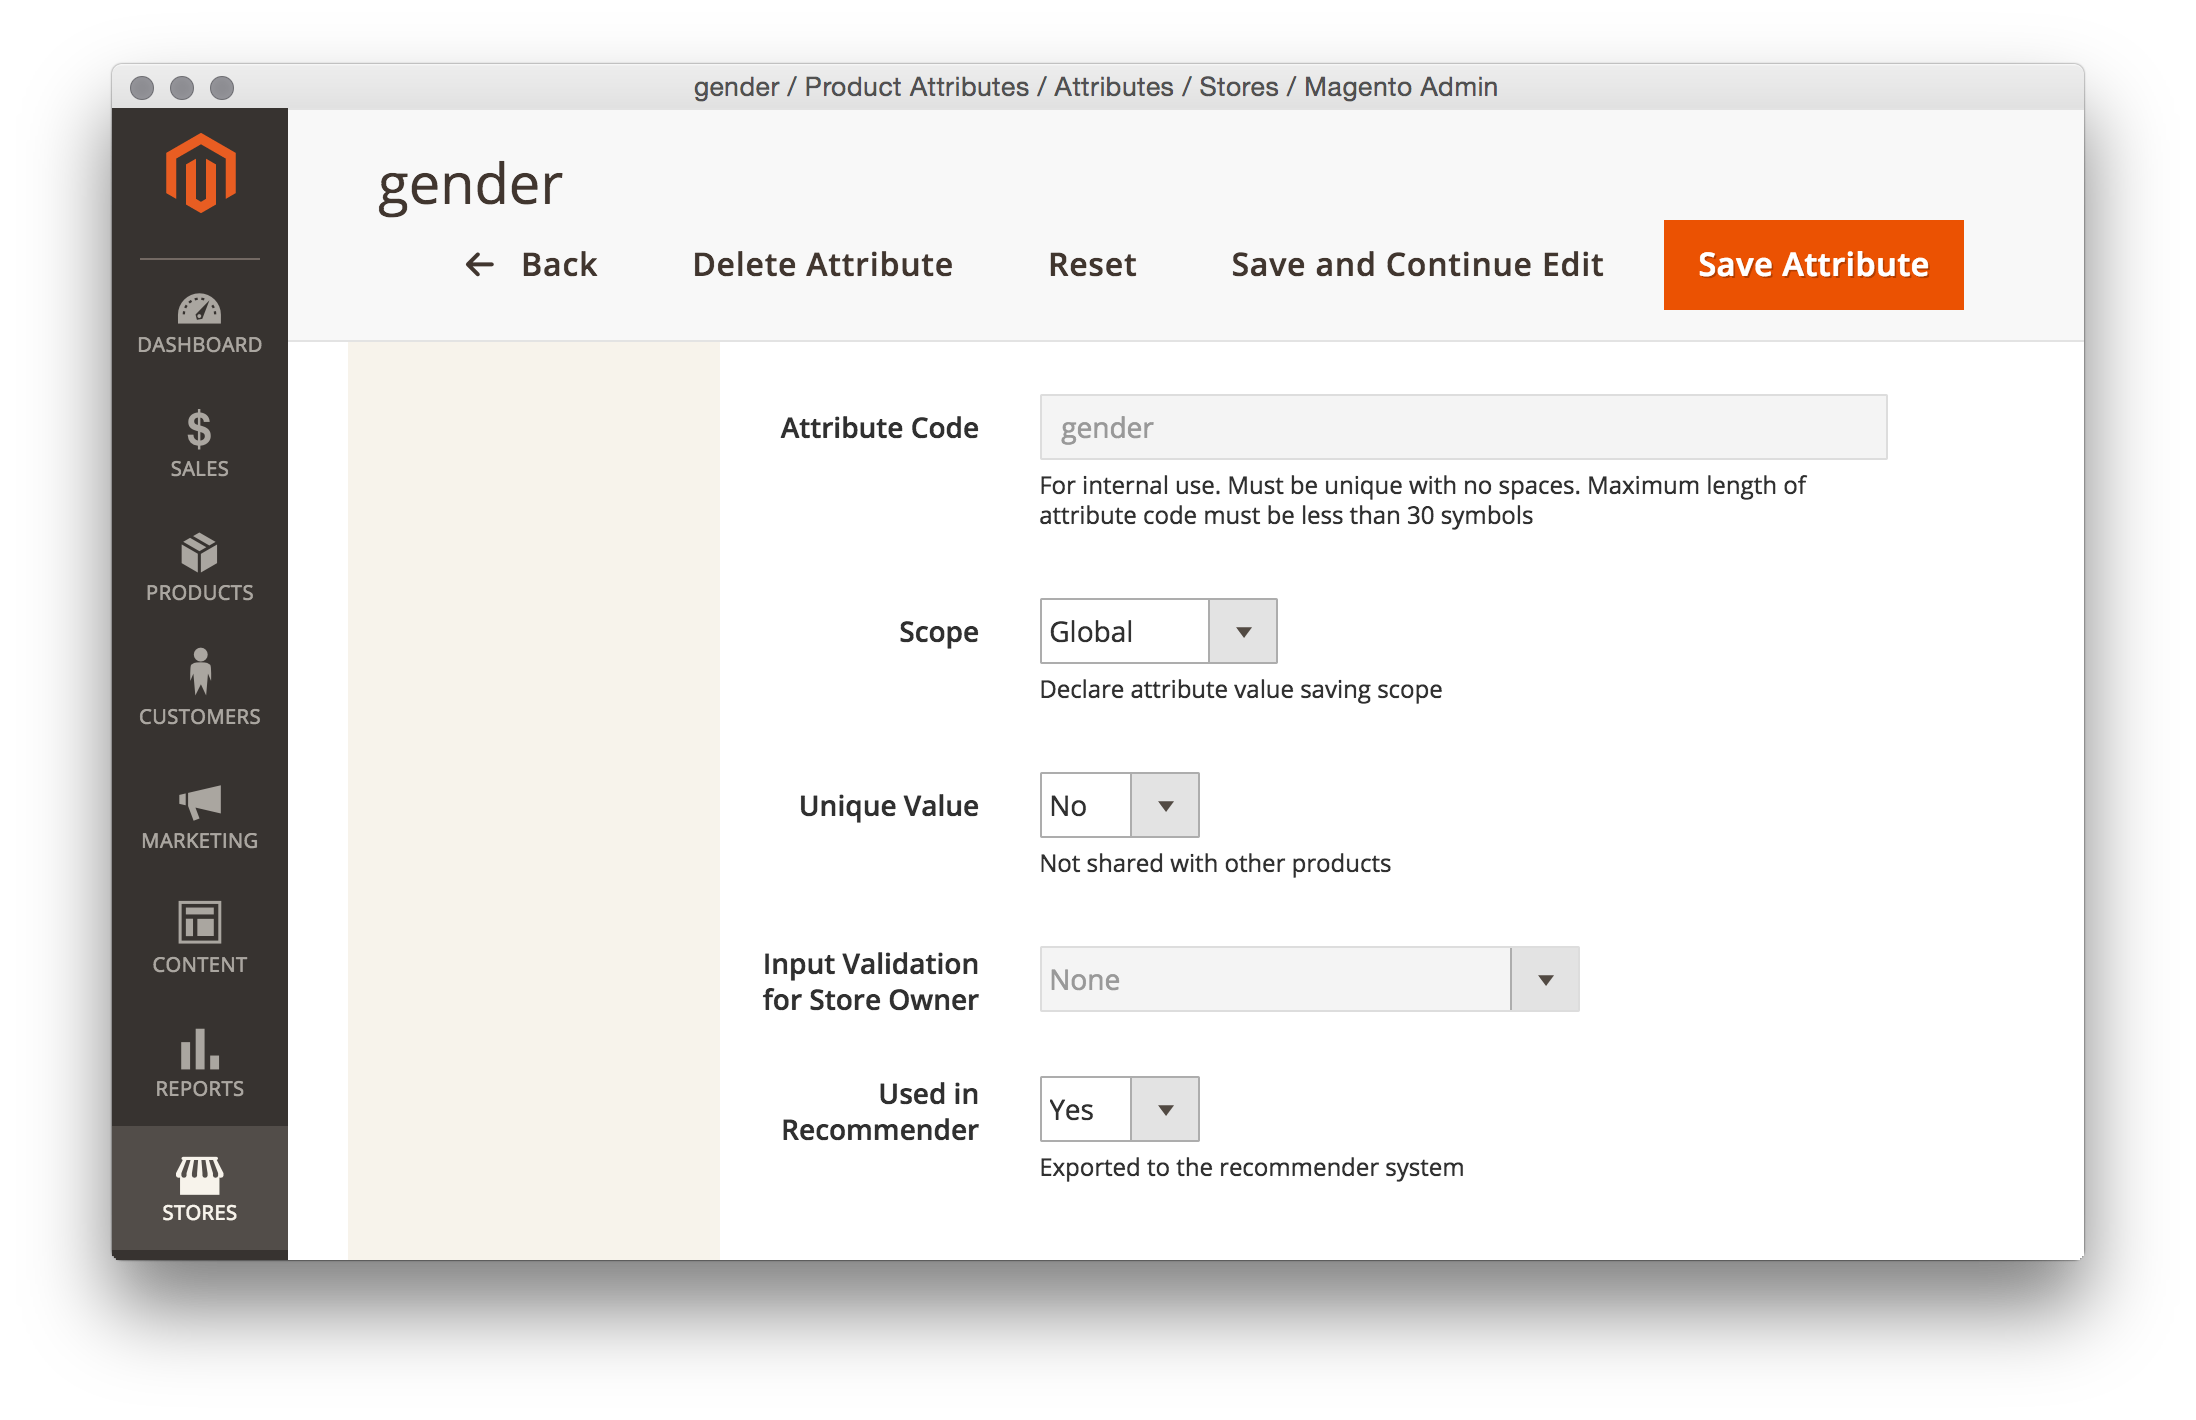
\includegraphics[width=\textwidth,center]{screens/masterdata.png}
    \caption{Master Data Management (Screenshot)}
    \label{fig:implementation-magento-master-data}
\end{figure}

Magento provides a user interface to manage these attributes and attribute sets; thus means that the master data can vary extensively between Magento instances. There are \emph{system attributes} which remain the same on any Magento instance but the majority of the relevant data would be merchant-specific. To accommodate this, the demo project implements a way for the merchant to mark attributes as \emph{``Used in Recommender''} which are to be exported to the framework, as shown in figure \ref{fig:implementation-magento-master-data}. However, as the demo project relies on the sample data generator of Magento to create attributes, setting that mark had to happen dynamically. The sample data generator and its static source data known as \emph{fixtures} have been extended so that a fixture can be replaced by a customised version containing the \emph{``Used in Recommender''} mark.

\subsection{Recommendations}

The integration of recommendations has been implemented in three parts:

First, a thin \emph{client} has been written which performs the request and processes the responses to the recommendation API of the framework. All requests and responses are logged in a file for troubleshooting.

Second, a \emph{recommendation model} is implemented for each recommender configured in the framework such as \emph{viewed products} and \emph{similar items in basket}. The purpose of these model classes is to provide the IDs the recommendation should be based on -- e.g. current user ID for the \emph{viewed products} and product IDs in the basket for \emph{similar items in the basket}. This is based on the requirement that each recommendation is in relation to something. They do not know internals of how the recommendations work. They are derived from an abstract class, which reduces the code size of the individual model classes to a minimum. They return a product collection filtered by the product IDs from the recommendation response.

Third, a \emph{recommendation widget} is provided which handles the display of recommendations to the user. Magento widgets are re-usable, configurable blocks which can be placed on the website. The demo project makes use of a universal product listing widget and feeds it with the product collection provided by the recommendation class. Magento enables developers and merchants to customise the layout of their website in a flexible way. The demo project was able to place these widgets on existing pages by supplying short XML files. An exception is the widget on the homepage (seen in figure \ref{fig:implementation-magento-homepage}) as that page is managed by the \emph{content management (sub)system (CMS)} of Magento. Since the homepage is part of the sample data, a customised fixture has been provided, similar to those discussed in the previous section.

\begin{figure}[!ht]
    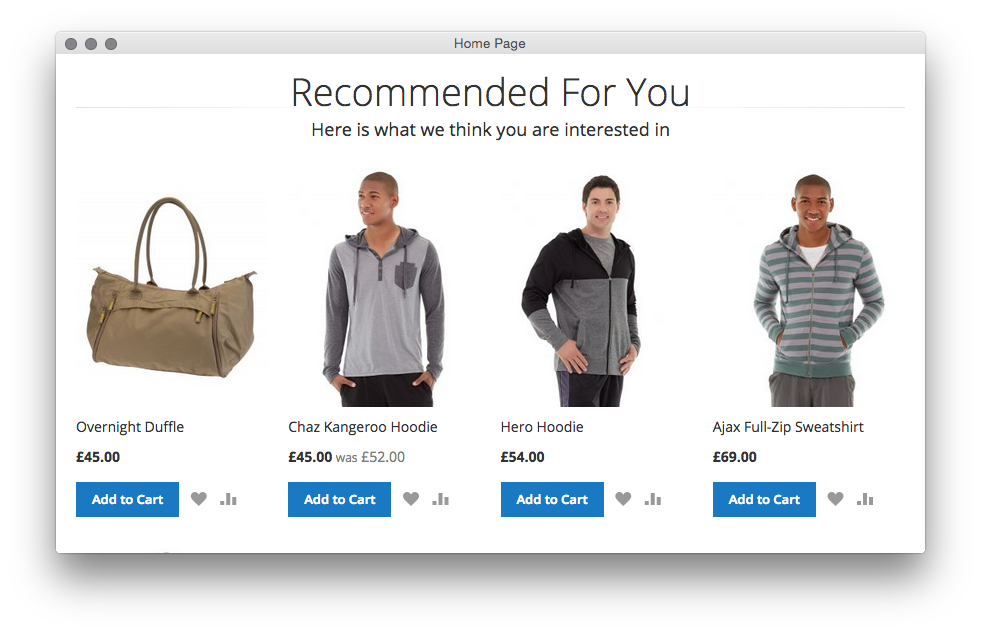
\includegraphics[width=\textwidth,center]{screens/homepage.png}
    \caption{Homepage Recommendations (Screenshot)}
    \label{fig:implementation-magento-homepage}
\end{figure}

\section{Provisioning}

Provisioning refers to the process of preparing an environment which fulfills the requirements to run systems and applications. It involves the installation of languages and libraries as well as proper configuration.

This project relies on the \emph{Linux} operating system and comes with provisioning instructions, which are outlined in the next sections.

\subsection{Virtualisation with Vagrant}

\emph{Vagrant} is a software system that manages virtual environments -- emulated computer systems also known as \emph{virtual machines} -- for development purposes. It enables a development team to standardise their development environments. This is in particular useful when the computer systems of developers vary from the computer system of the development environment -- e.g. a developer on \emph{Windows} working on a software running on Linux -- or among each other -- i.e. developers using different computer systems which would require provisioning instructions for all computer systems used. In order to run Vagrant, a single configuration file called \emph{Vagrantfile}, written in \emph{Ruby}, is added to the project's \emph{version control system} such as \emph{Git} and then shared with the team. A simple \texttt{vagrant up} command in a terminal is enough to boot up the machine.

Vagrant does not do the virtualisation itself but relies on established virtualisation software such as \emph{VirtualBox} and \emph{VMWare}. It also relies on so called \emph{boxes} -- a bare bone installation of a computer system minimally configured for Vagrant -- to bootstrap the virtual machine. Although the project works on any Linux distribution, due to the box requirement of Vagrant the Linux distribution \emph{Ubuntu} (version 14.04) has been used.

Another challenge was the fact that the sample data generator of \emph{Magento} is very inefficient and takes a few hours to complete. In order to reduce the provisioning time to a minimum, it was then decided to package a fully provisioned version of the development environment to a ready-to-go box. \emph{HashiCorp} -- the authors of Vagrant -- provide a service called \emph{Atlas} which allows such boxes to be uploaded and made publicly available. Boxes for VirtualBox and VMWare have been uploaded to Atlas since Vagrant boxes are specific to the virtualisation software used. It is rather important to notice that VMWare as well as its Vagrant provider -- the middleware between Vagrant and VMWare -- are both commercial whereas VirtualBox is open-source and free.

Vagrant also provides native support for configuration management software as discussed in the next section.

\subsection{Configuration Management with Puppet}

\emph{Puppet} is an open-source software system which manages the configuration of \emph{Microsoft Windows}, \emph{Linux} and other \emph{Unix}-like systems such as \emph{Mac OS X}. This is achieved by describing the expected system configuration in so-called \emph{manifest} files written in a custom declarative language derived from \emph{Ruby}. Upon execution, Puppet interprets these manifests into a configuration catalogue and compares it against the configuration of one or more new or existing systems. Differences noticed during that step are corrected by Puppet. This ensures the expected configuration on those systems and can be called repetitively.

Puppet supports writing manifests for more than one target environment. In fact, most companies are using Puppet to ensure the same configuration (with some variables) on multiple environments such as production, staging and development. In the Vagrant context the Puppet provisioning is called by default when a new virtual machine is created. However, it can also be called explicitly. Since this project utilises Puppet to provision a development environment only, the manifests are not ready for production. Ensuring that essential security measures, amongst others changing default passwords, were beyond the scope of this project.

Manifests can be grouped into so called Puppet \emph{modules}. \emph{PuppetLabs} -- the authors of Puppet - operate a community called \emph{PuppetForge} where modules are shared. This project utilised \emph{PuppetForge} modules e.g. for \emph{Apache} and \emph{PHP} where possible. In reality, most such modules are officially authored by PuppetLabs. Nonetheless, not all modules covered all the configuration needs of this project and were thus custom written inter alia for \emph{Magento}, \emph{Neo4j} as well as the \emph{framework} and \emph{recommender engines}. The Magento module builds dependencies, creates an Apache virtual host and a MySQL database and runs the Magento installer. The Neo4j module installs and configures the Neo4j server. The recommender module configures both framework and two recommender engines. It creates Apache virtual hosts, installs dependencies, creates \emph{Supervisor} programs to manage background processes and sets up \emph{Celery} and \emph{Flower}. External modules are integrated as Git \emph{submodules}. The provisioning source code in \ref{appendix-soure-code-provisioning} only lists manifests written by the project author.

Puppet can be understood as part of the \emph{infrastructure as code} or \emph{programmable infrastructure} initiatives in organisations. It enables version controlling and automation of provisioning infrastructure. Especially infrastructure based on \emph{cloud computing} and \emph{platform as a service (PaaS)} which involve many but constantly changing (e.g. auto-scaling) systems benefit from this. Alternatives to Puppet are \emph{Chef}, \emph{SaltStack} and \emph{Ansible}.

\subsection{Dependency Management}

Dependency management supports the declaration and installation of libraries a software system depends on. Whereas system package managers like \emph{Yum} and \emph{Apt} provide a system-wide solution for packages, dependency managers support versioned solution on a per-project basis. The latter is important as two pieces of software may depend on different versions of a dependency. Furthermore, dependency managers are usually tailored for a programming language and allow the distribution of libraries, which may not be available as a Yum or Apt package.

As mentioned in the abstract, this work relies on many open-source projects. It was since particularly important to separate own work from those third-party projects. For this, dependency managers were very essential. The framework relies on the Python dependency manager \emph{pip}. The \emph{Item-Similarity} engine as well as the demo application \emph{Magento} use the PHP dependency manager \emph{Composer} (Figure \ref{fig:implementation-provisioning-dependency}). Finally, the \emph{In-Common} engine utilises \emph{gom} which adds per-project capabilities to the overall self-sufficient \emph{Go} dependency manager.

\begin{figure}[!ht]
    \begin{minted}{js}
{
    // [...]
    "require": {
        "php": ">=5.5",
        "silex/silex": "~1.3",
        "neutron/mongo-odm-silex-provider": "0.1.3",
        "doctrine/mongodb-odm": "1.0.0-BETA13",
        "monolog/monolog": "^1.15"
    },
    "require-dev": {
        "symfony/browser-kit": "^2.7",
        "symfony/css-selector": "^2.7",
        "phpunit/phpunit": "4.7.*"
    },
    // [...]
}
    \end{minted}
    \caption{Composer Dependencies of Item-Similarity Engine (Code Listing)}
    \label{fig:implementation-provisioning-dependency}
\end{figure}